\documentclass[11pt]{article}
% Self-contained supplement; preamble mirrors death_of_a_chimera.tex so the sections
% below can be pasted into the manuscript (as appendices) without preamble changes.
\usepackage[margin=1in]{geometry}
\usepackage{amsmath,amssymb}
\usepackage{graphicx}
\usepackage{booktabs}
\usepackage{xcolor}
\usepackage[T1]{fontenc}
\usepackage{times}
\usepackage{microtype}
\graphicspath{{critical_review_figs/}{figures/}{paper_figures/}}

\newcommand{\kabs}{k_{\mathrm{abs}}}
\newcommand{\tabs}{\tau_{\mathrm{abs}}}
\newcommand{\Rincoh}{\overline{R}_{\mathrm{incoh}}}
\newcommand{\rhostd}{\rho_{\mathrm{std}}}

\title{\bfseries Supplementary material:\\ conditioning the aging hazard and validating
the chimera-death object}
\author{Avery Karlin}
\date{}

\begin{document}
\maketitle

\noindent
This supplement reports two run-first robustness analyses prompted by the two critical
questions a reader may raise about the headline statistical claims: (C1)~whether the
$A=0.5$ aging is a genuine state-level hazard or an artifact of pooling fixed transient
times across the seed ensemble, and (C2)~whether the nonlocal-ring chimera-death study's
increasing-hazard result is contaminated by a non-canonical decay channel or by the
choice of death criterion. Every number below is regenerated by committed scripts
(\texttt{critical\_review/} in the repository) and was independently reproduced with a
second, disjoint censored-Weibull implementation; no figure or value is a placeholder.
Section~\ref{supp:c1} concerns the two-population results of the main text directly;
Section~\ref{supp:c2} concerns the nonlocally-coupled ring (Wolfrum--Omel'chenko)
chimera-death campaign. Section~\ref{supp:insert} lists the short main-text sentences
these analyses license.

% =====================================================================
\section{Conditioning the $A=0.5$ aging on the collective initial condition}
\label{supp:c1}

At the operating corner the reduced flow is deterministic, so a censored-Weibull shape
$\kabs>1$ could in principle encode only the \emph{spread of fixed transient times} across
the random-seed ensemble (an initial-condition heterogeneity), rather than a hazard that
rises along each trajectory. We separate the two by stratifying the $200$-seed ensemble
at each population size into four equal-count bins of a collective initial-condition
coordinate and refitting the right-censored Weibull \emph{within} each stratum. We use
three independent stratifying variables: the initial inter-population phase gap
$|\Delta\phi_0|$; the initial incoherent-population order parameter
$\overline{R}_{\mathrm{incoh},0}$; and,
as the decisive test, the reduced three-variable model's \emph{predicted} lifetime
$t_{\mathrm{cap}}$ for that seed---which collapses the entire collective initial condition
onto its lifetime consequence, so that conditioning on it removes every lifetime
dependence the collective coordinates can express.

The aging survives conditioning in every case (Table~\ref{tab:c1}, Fig.~\ref{fig:c1}).
The pooled per-$N$ fits reproduce the main-text values $\kabs = 2.27,2.22,2.49,2.67,2.44,
2.72,3.03$ exactly. Within strata, $\kabs>1$ with $95\%$ profile-likelihood confidence
intervals excluding one in all $28$ (size~$\times$~bin) cells for each of the three
variables---$84/84$ cells in total---with $\kabs$ ranging from $1.88$ to $5.12$. The
within-bin coefficient of variation of $\tabs$ remains substantial ($0.22$--$0.56$, not a
degenerate spike) and tracks the fitted shape through the Weibull relation
$\mathrm{CV}(k)=\sqrt{\Gamma(1+2/k)/\Gamma(1+1/k)^2-1}$ (empirical-vs-predicted correlation
$0.996$), confirming a genuine aging-shaped within-stratum lifetime spread. Conditioning on
the reduced model's predicted lifetime---the strongest control available---leaves
$\kabs\in[2.00,5.00]$, again excluding one in all $28$ cells; within narrow predicted-lifetime
bands the shape if anything \emph{grows} with $N$, the opposite of a collective-IC confound.
This is consistent with the per-cycle ratchet of Sec.~5 (the per-pass hazard increment rises
from $0.031$ to $0.091$ across $N$, with the fraction of monotone-ratcheting runs reaching
unity by $N=32$): the hazard rises as the chimera ages regardless of where it started. We
note that at $A=0.5$ the censored fraction is exactly zero (all $1400$ runs absorb before
$t_{\max}=2000$\,s), so these are effectively uncensored maximum-likelihood fits.

\begin{table}[t]
\centering
\caption{Within-stratum aging at $A=0.5$. For each stratifying variable the seed
ensemble is split into four equal-count bins per $N$; a right-censored Weibull is fit
within each (size,\,bin) cell. ``CI excl.\ 1'' counts cells whose $95\%$
profile-likelihood interval on $\kabs$ lies above the memoryless value $k=1$.}
\label{tab:c1}
\begin{tabular}{lccc}
\toprule
stratifying variable & cells & $\kabs$ range & CI excl.\ 1 \\
\midrule
(pooled per-$N$, reference)              & 7  & $2.22$--$3.03$ & $7/7$ \\
$|\Delta\phi_0|$ (phase gap)             & 28 & $1.88$--$5.12$ & $28/28$ \\
$t_{\mathrm{cap}}$ (reduced pred.\ lifetime) & 28 & $2.00$--$5.00$ & $28/28$ \\
$\overline{R}_{\mathrm{incoh},0}$ (incoherent IC level) & 28 & $1.88$--$4.83$ & $28/28$ \\
\bottomrule
\end{tabular}
\end{table}

\begin{figure}[t]
\centering
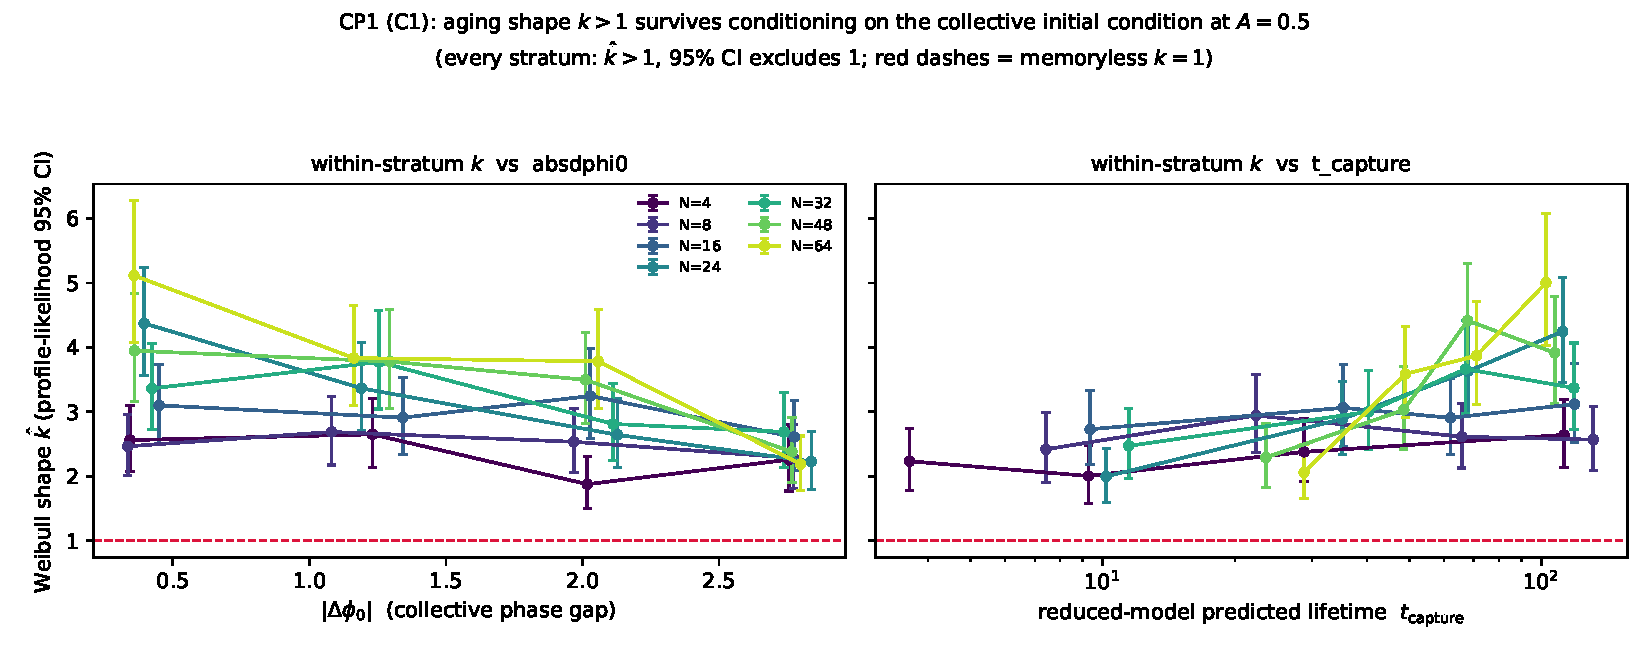
\includegraphics[width=0.95\linewidth]{cp1_stratified}
\caption{Aging survives conditioning on the collective initial condition at $A=0.5$.
Within-stratum censored-Weibull shape $\hat k$ (profile-likelihood $95\%$ intervals)
versus bin, one curve per population size $N$, for stratification by $|\Delta\phi_0|$
(left) and by the reduced model's predicted lifetime $t_{\mathrm{cap}}$ (right). Every
stratum sits above the memoryless value $k=1$ (red dashes); within a fixed collective
initial condition the lifetime distribution keeps an increasing-hazard shape, so the
aging is a property of the trajectory, not of the initial-condition ensemble.}
\label{fig:c1}
\end{figure}

% =====================================================================
\section{The dying ring object and its criterion-independence}
\label{supp:c2}

The nonlocal-ring chimera-death campaign reports a Weibull shape that saturates to a
finite $k_\infty\approx1.35$--$1.65>1$ as $N\!\to\!\infty$ (per-$\beta$ bootstrap
intervals excluding one). Two features invite scrutiny. First, the median ring lifetime
\emph{decreases} with $N$ in the studied window---opposite to the lifetime growth of the
deep-stable regime~[Wolfrum \& Omel'chenko, Phys.\ Rev.\ E \textbf{84}, 015201(R)
(2011)]---raising the worry that the death criterion ($\rhostd(t)<0.04$ held for $50$
time units, where $\rhostd$ is the spatial standard deviation of the local order
parameter $\rho_k$) times a non-canonical decay channel. Second, the increasing-hazard
shape might be specific to that criterion. We address both directly; both survive.

\paragraph{The object being killed is a canonical chimera (97--98\%).} The spatial field
$\rho_k(t,\cdot)$ was not stored, but every run is exactly reproducible from its logged
seed, so we re-ran all $300$ trajectories per cell at $N=256$ for $\beta=0.110$ and
$\beta=0.130$ with field dumping; the re-detected lifetimes reproduce the campaign values
bit-for-bit ($0/600$ mismatches). Classifying each pre-death state by its spatial
structure (a contrast gate on $\rhostd$ together with the dominant spatial Fourier mode of
$\rho_k$, which is drift invariant) gives the breakdown in Table~\ref{tab:c2a}. The death
criterion times the collapse of a genuine chimera---one contiguous coherent arc plus one
incoherent arc, or a multi-headed variant---in $98.0\%$ ($\beta=0.110$) and $97.3\%$
($\beta=0.130$) of runs; the degenerate ``dissolve-then-linger'' channel (the chimera
disperses early and a low-contrast state persists until full homogenisation) is real but
rare, $2.0$--$2.7\%$. Refitting after removing it leaves the Weibull shape unchanged---if
anything slightly larger---with intervals still excluding one (Table~\ref{tab:c2a});
sweeping the contrast gate over $[0.06,0.12]$ only moves $\hat k$ further from one. The
$k_\infty$ claim is therefore not an artifact of the rare degenerate channel.

\paragraph{The trend and the hazard shape are criterion-independent.} Re-detecting death
on the same $\beta=0.130$ trajectories under alternative literature-style criteria, the
median lifetime \emph{decreases} with $N$ under every one (Table~\ref{tab:c2b}, left;
$\tilde\tau(256)/\tilde\tau(32)=0.34$--$0.40$), so the inversion is a property of the
near-boundary dynamics, not of the detector. The increasing-hazard shape $\hat k(N)>1$ is
likewise robust under the structure-loss criteria ($\rhostd$ below $0.08$ or $0.10$;
Table~\ref{tab:c2b}, right; all intervals exclude one, with $0\%$ censoring). A
mean-coherence-level criterion ($\rho$-mean above a fixed value) appears to drive
$\hat k$ below one at large $N$, but this is a diagnosed censoring artifact: $6.7\%$ of
the $N=256$ collapses go to a spatially uniform \emph{twisted} state ($\rho_k\approx0.50$,
genuinely dead by $\rhostd<0.04$ at finite time) rather than the high-coherence sync
plateau, and a mean-coherence threshold mislabels these genuine deaths as censored,
injecting a spurious immortal tail; re-timing them at their true death restores
$\hat k(N)=1.26,1.44,1.62,1.54,1.57$, all intervals above one. An independent
Kaplan--Meier log-cumulative-hazard slope ($1.5$--$2.1$ across $N$) corroborates the
increasing hazard without any Weibull fit. That the spatial-homogeneity criterion---unlike
a coherence-level threshold---captures both the synchronised and the twisted collapse
channels is itself a reason to prefer it.

\begin{table}[t]
\centering
\caption{Pre-death object at $N=256$ ($300$ runs per cell). ``chimera death'' is the sum
of single-arc and multi-headed chimera collapses. $\hat k$ columns are right-censored
Weibull shapes (profile-likelihood $95\%$ intervals) on all runs, on chimera deaths only,
and on single-arc deaths only.}
\label{tab:c2a}
\footnotesize
\setlength{\tabcolsep}{4pt}
\begin{tabular}{lccccccc}
\toprule
& single-arc & multi-head & degen.\ & chim.\ death & $\hat k$ all & $\hat k$ chim.\ & $\hat k$ single \\
\midrule
$\beta=0.110$ & $83.7\%$ & $14.3\%$ & $2.0\%$ & $98.0\%$ & $1.22\,[1.12,1.32]$ & $1.24\,[1.14,1.35]$ & $1.24\,[1.13,1.36]$ \\
$\beta=0.130$ & $89.3\%$ & $8.0\%$  & $2.7\%$ & $97.3\%$ & $1.47\,[1.35,1.58]$ & $1.48\,[1.36,1.60]$ & $1.46\,[1.34,1.59]$ \\
\bottomrule
\end{tabular}
\end{table}

\begin{table}[t]
\centering
\caption{Criterion-independence at $\beta=0.130$. Median lifetime $\tilde\tau$ (left) and
Weibull shape $\hat k$ (right) versus $N$, re-detected on the same trajectories under each
criterion. ``mean-coh (corr.)'' re-times the twisted-state collapses the raw
mean-coherence rule mislabels as censored. All $\rhostd$-based criteria carry $0\%$
censoring.}
\label{tab:c2b}
\small
\setlength{\tabcolsep}{4pt}
\begin{tabular}{lccccc@{\quad}ccccc}
\toprule
& \multicolumn{5}{c}{median $\tilde\tau(N)$} & \multicolumn{5}{c}{$\hat k(N)$} \\
\cmidrule(r){2-6}\cmidrule(l){7-11}
criterion & 32 & 64 & 128 & 192 & 256 & 32 & 64 & 128 & 192 & 256 \\
\midrule
$\rhostd<0.04$ (orig.)   & 872 & 422 & 404 & 349 & 345 & 1.33 & 1.55 & 1.68 & 1.68 & 1.47 \\
$\rhostd<0.08$           & 828 & 383 & 372 & 314 & 308 & 1.28 & 1.45 & 1.61 & 1.56 & 1.42 \\
$\rhostd<0.10$           & 815 & 372 & 356 & 303 & 289 & 1.26 & 1.41 & 1.59 & 1.50 & 1.40 \\
mean-coh (corr.)         & 810 & 379 & 362 & 310 & 276 & 1.26 & 1.44 & 1.62 & 1.54 & 1.57 \\
\bottomrule
\end{tabular}
\end{table}

\begin{figure}[t]
\centering
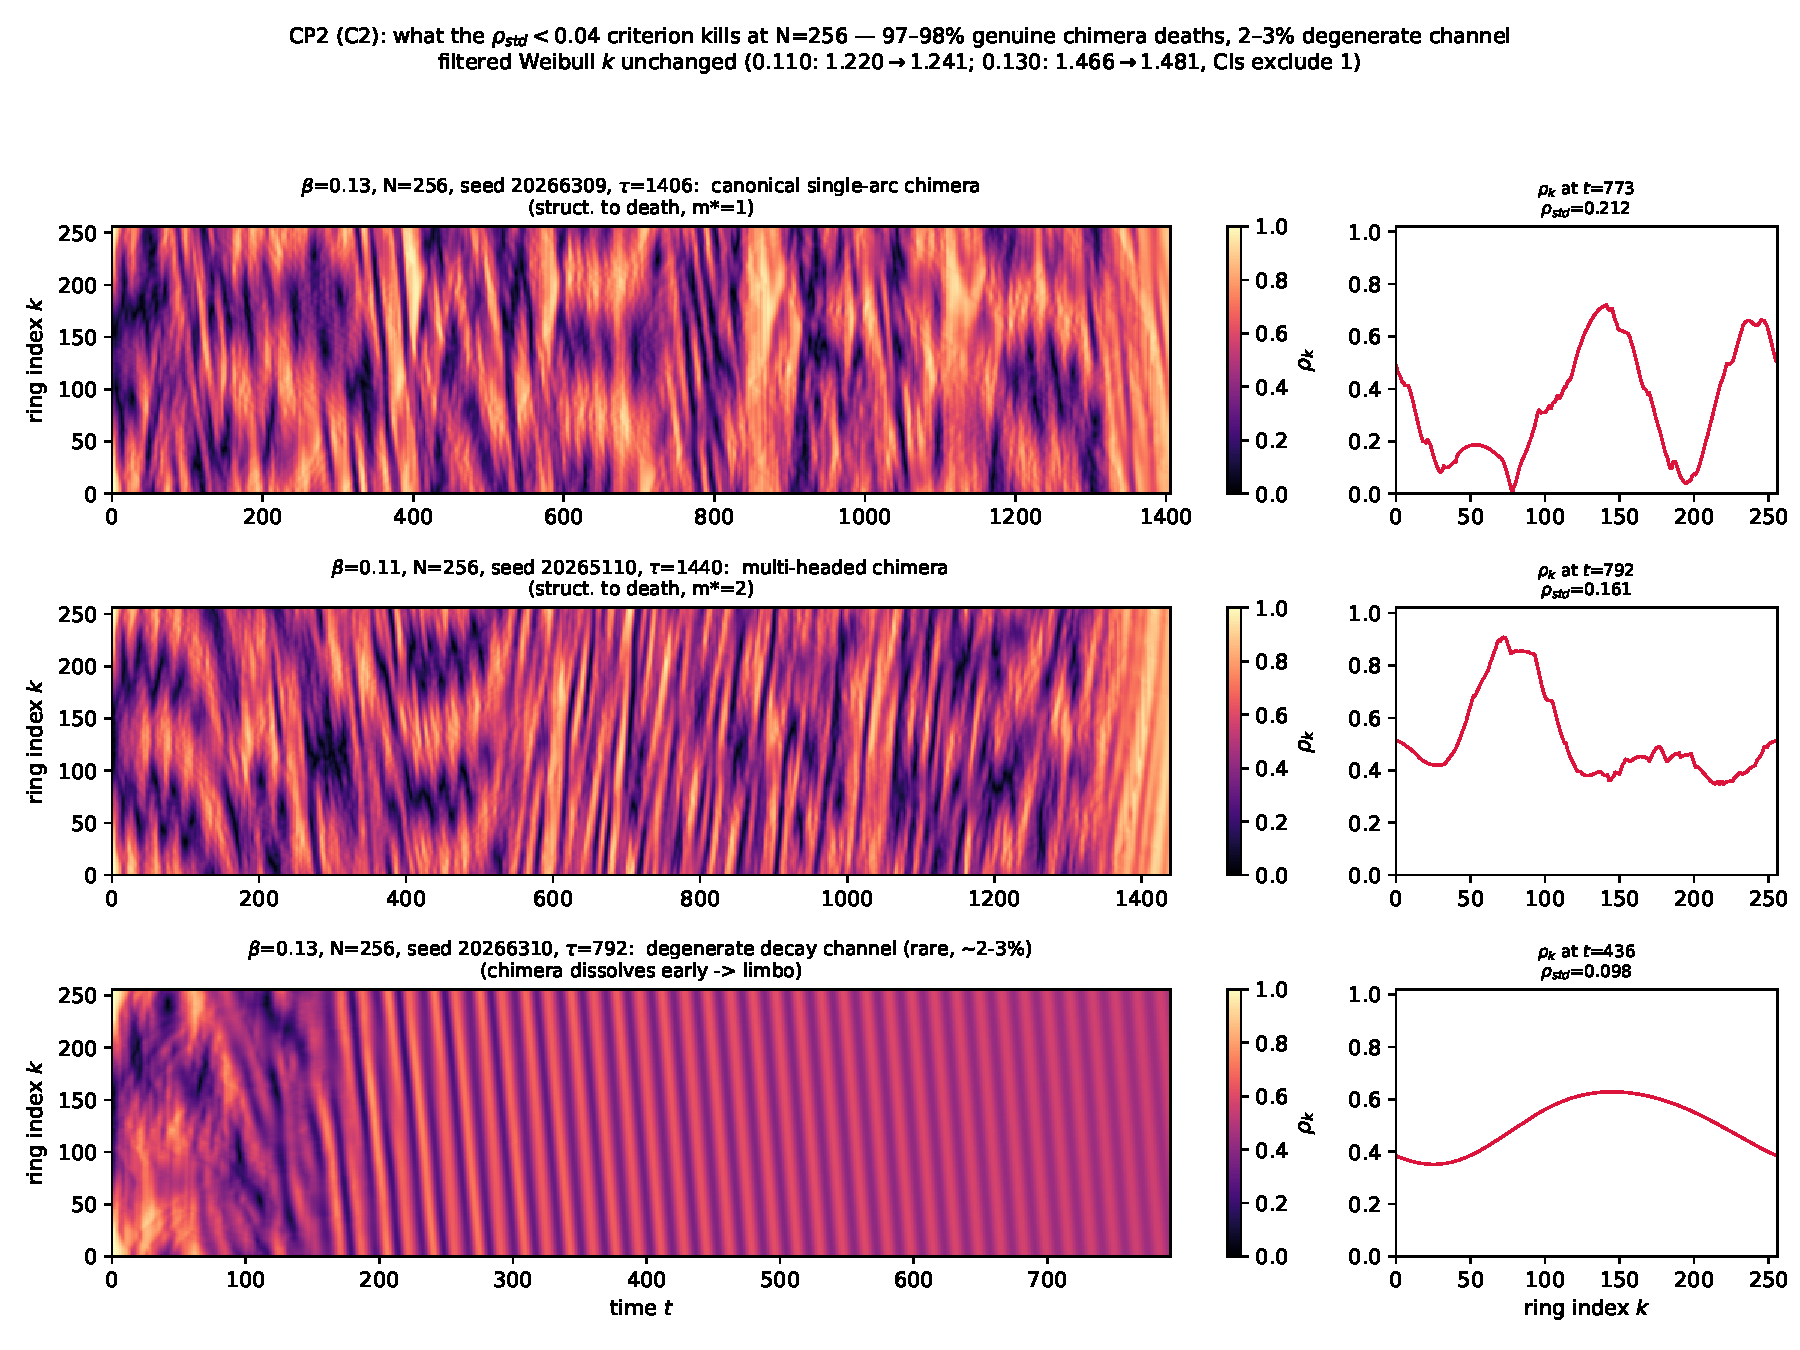
\includegraphics[width=0.92\linewidth]{cp2_object}
\caption{What the $\rhostd<0.04$ criterion kills at $N=256$. Space--time local-coherence
fields $\rho_k(t,k)$ (left) with a representative mature snapshot (right) for the three
pre-death behaviours: a canonical single-arc chimera (top, structured to death), a
multi-headed chimera (middle), and the rare degenerate channel (bottom, the chimera
disperses early and a low-contrast state lingers). $97$--$98\%$ of deaths are of the first
two (genuine chimera) type; removing the degenerate channel leaves the Weibull shape
unchanged.}
\label{fig:c2a}
\end{figure}

\begin{figure}[t]
\centering
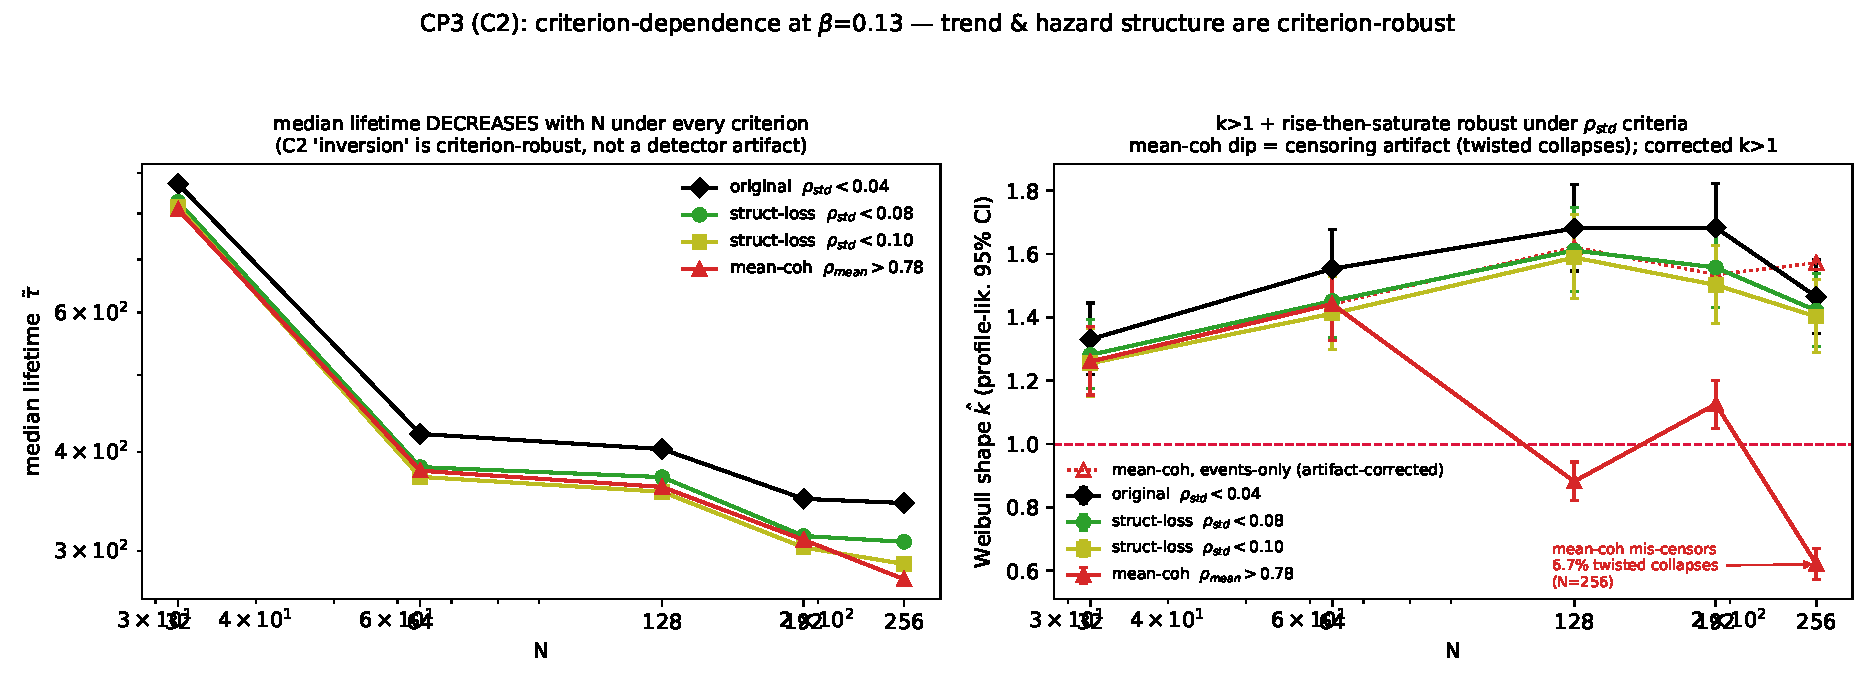
\includegraphics[width=0.92\linewidth]{cp3_criterion}
\caption{Criterion-independence at $\beta=0.130$. Left: median lifetime decreases with $N$
under every death criterion (the near-boundary inversion is not a detector artifact).
Right: the Weibull shape $\hat k(N)$ stays above one under the spatial-homogeneity
($\rhostd$) criteria; the mean-coherence rule's apparent dip below one at large $N$ is a
censoring artifact (twisted-state collapses mislabelled as censored), and the
artifact-corrected curve (open markers) returns above one.}
\label{fig:c2b}
\end{figure}

% =====================================================================
\section{Suggested main-text insertions}
\label{supp:insert}

These analyses license the following short additions, kept deliberately minimal.

\paragraph{For Sec.~4 (Aging), after the $\kabs$ values.} ``This aging is not an artifact
of pooling heterogeneous deterministic transients: stratifying the seed ensemble by the
collective initial condition---the inter-population phase gap, the incoherent-population
level, or the reduced model's predicted lifetime---and refitting within each stratum
leaves $\kabs>1$ with confidence intervals excluding one in all $84$ size$\times$stratum
cells, and the within-stratum lifetime spread retains an increasing-hazard shape
(Supplement, Sec.~\ref{supp:c1}).''

\paragraph{For the ring-reframe / Discussion treatment of the nonlocal ring.} ``The
decreasing ring median lifetime with $N$ at these near-boundary $\beta$ reflects the
near-collapse side of the existence boundary rather than the deep-stable regime of
Wolfrum--Omel'chenko, in which lifetimes grow with $N$; the dying object is a canonical
(single- or multi-arc) chimera in $97$--$98\%$ of runs, and the increasing-hazard shape
$k(N)>1$ is robust to the death criterion and to the rare degenerate decay channel
(Supplement, Sec.~\ref{supp:c2}).''

\paragraph{Methods/Data-availability note.} ``Stratified-hazard and criterion-robustness
analyses, including the field re-runs validating the dying object, are in
\texttt{critical\_review/} and were independently reproduced with a disjoint
censored-Weibull implementation.''

\end{document}
